\documentclass[hidelinks]{acaces}


%%%%%%%%%%%%%%%%%%%%%%%%%
%% Document and Layout %%
%%%%%%%%%%%%%%%%%%%%%%%%%

% Fix for multiple "No room for a new \dimen" errors.
%
% See: http://tex.stackexchange.com/questions/38607/no-room-for-a-new-dimen
%
\usepackage{etex}

% Fix for "'babel/polyglossia' detected but 'csquotes' missing"
% warning. NOTE: Include after inputenc.
%
\usepackage{csquotes}
\usepackage{booktabs}

% Required for full page-width tables.
\usepackage{tabularx}

\usepackage{wrapfig}

\usepackage{adjustbox}

% Define column types L, C, R with known text justification and fixed
% widths:
\usepackage{array}
\newcolumntype{L}[1]{>{\raggedright\let\newline\\\arraybackslash\hspace{0pt}}m{#1}}
\newcolumntype{C}[1]{>{\centering\let\newline\\\arraybackslash\hspace{0pt}}m{#1}}
\newcolumntype{R}[1]{>{\raggedleft\let\newline\\\arraybackslash\hspace{0pt}}m{#1}}

% Make internal macro definitions accessible,
% e.g. \@title, \@date \@author.
\makeatletter

%%%%%%%%%%%%%%%%%%%%%
% Table of Contents %
%%%%%%%%%%%%%%%%%%%%%

\usepackage{color}
\newcommand{\fix}[1]{\textcolor{red}{\em\footnotesize#1}}


%%%%%%%%%%%%%%%%
% Bibliography %
%%%%%%%%%%%%%%%%
\usepackage[%
    backend=biber,%bibtex,
    style=numeric-comp,
    % style=numeric-comp,  % numerical-compressed
    sorting=none,        % nty,nyt,nyvt,anyt,anyvt,ynt,ydnt,none
    sortcites=true,      % sort \cite{b a d c}: true,false
    block=none,          % space between blocks: none,space,par,nbpar,ragged
    indexing=false,      % indexing options: true,false,cite,bib
    citereset=none,      % don't reset cites
    isbn=false,          % print ISBN?
    url=true,            % print URL?
    doi=false,           % print DOI?
    natbib=true,         % natbib compatability
    maxbibnames=99       % no 'et-al' in the bibliography pls
  ]{biblatex}

\addbibresource{refs.bib}

% Reduce the font size of the bibliography:
\renewcommand{\bibfont}{\normalfont\scriptsize}

\usepackage{setspace}
\onehalfspacing


%%%%%%%%%%%%%%%%%%%%%%%%%%%%%%%%%%%%%
%% Figures, footnotes and listings %%
%%%%%%%%%%%%%%%%%%%%%%%%%%%%%%%%%%%%%

% Pre-requisites for rendering upquotes in listings package.
\usepackage[T1]{fontenc}
\usepackage{lmodern}
\usepackage{textcomp}

% Pseudo-code listings.
\usepackage{algorithm}
\usepackage{algpseudocode}
\newcommand{\Break}{\State \textbf{break} }
\algblockdefx[Loop]{Loop}{EndLoop}[1][]{\textbf{Loop} #1}{\textbf{End
    Loop}}

\algrenewcommand\ALG@beginalgorithmic{\footnotesize}


%%%%%%%%%%%%%%%%%%%%%%%%
%% Graphics and maths %%
%%%%%%%%%%%%%%%%%%%%%%%%
\usepackage{amsmath}

% Vector notation, e.g. \vv{x}:
%
\usepackage{esvect}

% Additional amsmath symbols, see:
%
% http://texblog.org/2007/08/27/number-sets-prime-natural-integer-rational-real-and-complex-in-latex/
%
\usepackage{amsfonts}
\usepackage{amssymb}

\usepackage{graphicx}
\usepackage{mathtools}

% Provide bold font face in maths.
\usepackage{bm}

\usepackage{subcaption}
\expandafter\def\csname ver@subfig.sty\endcsname{}

% Define an 'myalignat' command which behave as 'alignat' without the
% vertical top and bottom padding. See:
%     http://www.latex-community.org/forum/viewtopic.php?f=5&t=1890
\newenvironment{myalignat}[1]{%
  \setlength{\abovedisplayskip}{-.7\baselineskip}%
  \setlength{\abovedisplayshortskip}{\abovedisplayskip}%
  \start@align\z@\st@rredtrue#1
}%
{\endalign}

% Define additional operators:
\DeclareMathOperator*{\argmin}{arg\,min}
\DeclareMathOperator*{\argmax}{arg\,max}

\DeclareMathOperator*{\gain}{Gain}

% Skeleton operators.
\DeclareMathOperator*{\map}{Map}
\DeclareMathOperator*{\reduce}{Reduce}
\DeclareMathOperator*{\scan}{Scan}
\DeclareMathOperator*{\stencil}{Stencil}
\DeclareMathOperator*{\zip}{Zip}
\DeclareMathOperator*{\allpairs}{All\,Pairs}

% Define a command to allow word breaking.
\newcommand*\wrapletters[1]{\wr@pletters#1\@nil}
\def\wr@pletters#1#2\@nil{#1\allowbreak\if&#2&\else\wr@pletters#2\@nil\fi}

% Define a command to create centred page titles.
\newcommand{\centredtitle}[1]{
  \begin{center}
    \large
    \vspace{0.9cm}
    \textbf{#1}
  \end{center}}

% Provide generic commands \degree, \celsius, \perthousand, \micro
% and \ohm which work both in text and maths mode.
\usepackage{gensymb}

\begin{document}

\title{Autotuning OpenCL Workgroup Sizes}

\author{
Chris~Cummins\addressnum{1},
Pavlos~Petoumenos\addressnum{1},
Michel~Steuwer\addressnum{1},
Hugh~Leather\addressnum{1}
}

\address{1}{
University of Edinburgh,
UK
}

\extra{1}{% Contacts
  E-mail: c.cummins@ed.ac.uk, ppetoume@inf.ed.ac.uk,
  michel.steuwer@ed.ac.uk, hleather@inf.ed.ac.uk%
}%
\extra{2}{% Acknowledgements
  This work was supported by the UK EPSRC under grants EP/L01503X/1
  (CDT in Pervasive Parallelism), EP/H044752/1 (ALEA), and
  EP/M015793/1 (DIVIDEND).%
}

\pagestyle{empty}


\begin{abstract}
  Selecting appropriate workgroup sizes for OpenCL is critical for
  program performance, and requires knowledge of the underlying
  hardware, the data being operated on, and the kernel
  implementation. We propose the use of machine learning-enabled
  autotuning to automatically predict workgroup sizes for stencil
  patterns on CPUs and multi-GPUs, using the Algorithmic Skeleton
  library SkelCL. In an evaluation across 429 combinations of
  architecture, kernel, and dataset, we find that static tuning of
  workgroup size achieves only $26\%$ of the optimal
  performance. Using machine learning and synthetically generated
  stencil programs, we achieve $92\%$ of this maximum, demonstrating a
  median $3.79\times$ speedup over the best possible fixed workgroup
  size.
\end{abstract}

\vspace{-.5em}
\keywords{%
  OpenCL; %
  Autotuning; %
  Stencil codes; %
  GPUs; %
  Machine learning; %
  Synthetic benchmarking%
}

\vspace{-2em}
\section{Introduction}

Efficient, tuned implementations of stencil codes are highly sought
after, with a variety of applications from fluid dynamics to quantum
mechanics. OpenCL enables the application of a range of heterogeneous
devices to parallelise stencils; however, achieving portable
performance is a hard task --- OpenCL kernels are sensitive to
properties of the underlying hardware, to the implementation, and even
to the dataset that is operated upon. This forces developers to
laboriously hand tune performance on a case-by-case basis, since
simple heuristics fail to exploit the available performance. Iterative
search approaches have been shown to select good
values~\cite{Nugteren2015,Ansel2013,Zhang2013a}, but these processes
are expensive and must be repeated for every new program or change to
hardware and dataset. In this work we demonstrate how machine
learning-enabled autotuning can be applied to Algorithmic Skeletons to
achieve near optimal performance of unseen stencils operations,
without requiring hand tuning or iterative searches.

\section{The SkelCL Stencil Pattern}

\begin{wrapfigure}{r}{0.38\textwidth}
% \vspace{-3em}
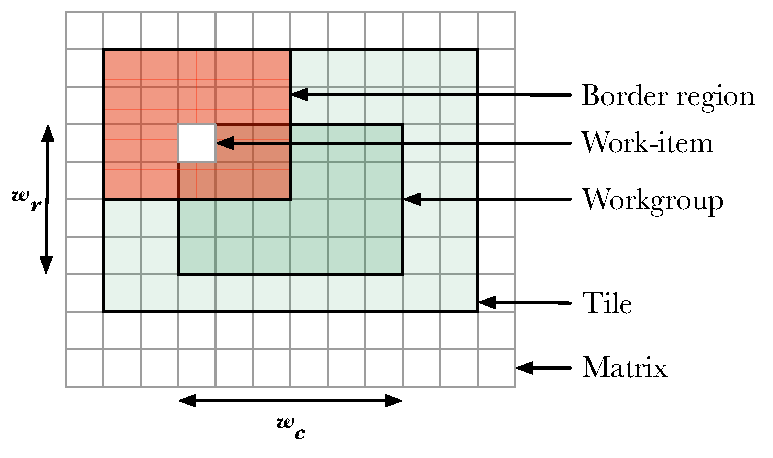
\includegraphics[width=.38\textwidth]{stencil}
\caption[Stencil border region]{%
  The execution of a stencil: an input matrix is decomposed into
  workgroups, and elements within workgroups are mapped to work-items.
  The values used by workgroups are mapped to local memory.%
  \vspace{-.75em} }
\label{fig:stencil-shape}
\end{wrapfigure}

SkelCL is an Algorithmic Skeleton library which provides OpenCL
implementations of data parallel patterns for heterogeneous
parallelism using CPUs and
multi-GPUs~\cite{Steuwer2011}. Figure~\ref{fig:stencil-shape} shows
the components of the SkelCL stencil pattern, which applies a
user-provided \emph{customising function} to each element of a 2D
matrix. The value of each element is updated based on its current
value and the value of one or more neighbouring elements, called the
\emph{border region}. When a SkelCL stencil pattern is executed, each
of the matrix elements are mapped to OpenCL work-items; and this
collection of work-items is divided into \emph{workgroups} for
execution on the target hardware. A \emph{tile} of elements the size
of the workgroup and the perimeter border region is allocated in local
memory for use by work-items. Changing the workgroup size affects both
the number of workgroups which can be active simultaneously, and the
amount of local memory required for each workgroup. While the user
defines the size, type, and border region of the matrix being operated
upon, it is the responsibility of the SkelCL implementation to select
an appropriate workgroup size to use.

\section{OpenCL Workgroup Size Optimization Space}

Preliminary experiments demonstrated that selection of an appropriate
workgroup size $w$ from the space of all possible workgroup sizes
$w \in W$ depends on properties of the kernel, hardware, and dataset,
illustrated in Figures~\ref{fig:motivation-arch}
and~\ref{fig:motivation-prog}. Additionally, the optimisation space is
subject to hard constraints which cannot conveniently be statically
determined. Each OpenCL device and kernel imposes a maximum workgroup
size determined by the hardware resources and resource requirements of
a program. Preliminary experiments found that not all points in the
workgroup size space provide correct programs, even if they satisfy
the kernel and architectural constraints. We call these points in the
space \emph{refused parameters}. For a given \emph{scenario} $s$ (a
combination of program, device, and dataset), we define a
\textit{legal} workgroup size as one which satisfies the architectural
and kernel constraints $w < W_{max}(s)$ and is not refused
$w \notin W_{refused}(s)$. The subset of legal workgroup sizes for a
given scenario $W_{legal}(s) \subset W$ is then:
%
\begin{equation}
  W_{legal}(s) \subset W = \left\{w | w \in W, w < W_{\max}(s) \right\} - W_{refused}(s)
\end{equation}


\begin{figure}
\centering
\adjustbox{valign=t}{%
  \begin{minipage}{.48\textwidth}
    \centering
    \begin{subfigure}[h]{.48\columnwidth}
      \centering
      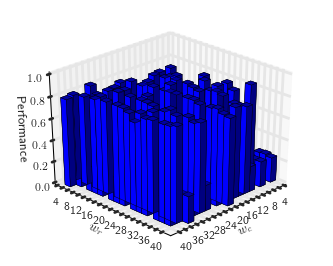
\includegraphics[width=1.0\columnwidth]{motivation_1}
      \vspace{-1.5em} % Shrink vertical padding
      \caption{}
      \label{fig:motivation-1}
    \end{subfigure}
    ~%
    \begin{subfigure}[h]{.48\columnwidth}
      \centering
      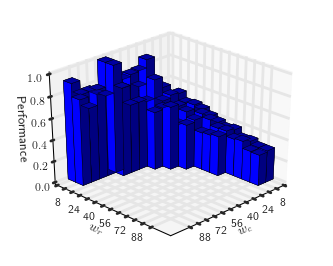
\includegraphics[width=1.0\columnwidth]{motivation_2}
      \vspace{-1.5em} % Shrink vertical padding
      \caption{}
      \label{fig:motivation-2}
    \end{subfigure}
    \caption{%
      The performance of different workgroup sizes for the same
      stencil program on two different devices:
      (\subref{fig:motivation-1}) Intel CPU,
      (\subref{fig:motivation-2}) NVIDIA GPU.%
    }
    \label{fig:motivation-arch}
  \end{minipage}%
}%
\hspace{2.5mm}
\adjustbox{valign=t}{%
  \begin{minipage}{.48\textwidth}
    \centering
    \begin{subfigure}[h]{.48\columnwidth}
      \centering
      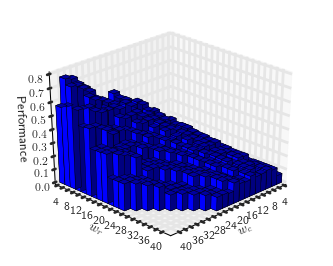
\includegraphics[width=1.0\columnwidth]{motivation_3}
      \vspace{-1.5em} % Shrink vertical padding
      \caption{}
      \label{fig:motivation-3}
    \end{subfigure}
    ~%
    \begin{subfigure}[h]{.48\columnwidth}
      \centering
      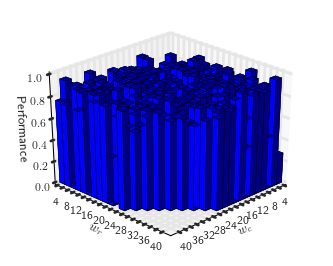
\includegraphics[width=1.0\columnwidth]{motivation_4}
      \vspace{-1.5em} % Shrink vertical padding
      \caption{}
      \label{fig:motivation-4}
    \end{subfigure}
    \caption{%
      The performance of different workgroup sizes for the same device
      executing two different stencil programs.%
    }
    \label{fig:motivation-prog}
  \end{minipage}%
}
\end{figure}


\section{Autotuning Methodology}

The goal of our machine learning-enabled autotuner is to predict, for
a given scenario, the workgroup size that will provide the shortest
runtime.
%
% The goal of machine learning enabled autotuning is to predict, for a
% given scenario $s$, the workgroup size $f(s)$ that will provide the
% shortest runtime $t(s, w)$:
% %
% \begin{equation}
%   f(s) = \underset{w \in W_{legal(s)}}{\argmin} t(s,w)
% \end{equation}
% %
The OpenCL workgroup size optimization space is large, complex, and
non-linear. Successfully applying machine learning to this problem
requires plentiful training data, the careful selection of explanatory
variables, and appropriate machine learning methods:
%
\vspace{-1.2em}
\paragraph{Explanatory variables} 102 variables are extracted to
capture information about the device, program, and dataset of a
scenario. Device variables capture information about the host and
target hardware (e.g.\ number of compute units, local memory size,
cache sizes). Program variables include static instruction densities,
the total number of basic blocks, and the total instruction
count. Dataset variables include the data types (input and output),
and dimensions of the input matrix and stencil region.
%
\vspace{-1.2em}
\paragraph{Training Data} A parameterised template substitution engine
is used to generate synthetic stencil programs. To generate training
data, these synthetically generated programs are executed on a range
of different execution devices, using different datasets, and
exhaustively enumerating the legal workgroup sizes. The workgroup size
which gives the best performance for each particular device, program,
and dataset is combined with the explanatory variables to create
training data.
%
\vspace{-1.2em}
\paragraph{Classification} Our approach uses a J48 Decision Tree
classifier~\cite{Han2011}, due to its low runtime cost and ability to
efficiently handle large dimensionality training data. In training,
the classifier correlate patterns between explanatory variables and
the workgroup sizes which provide optimal performance. After training,
it predicts the workgroup size for new sets of explanatory
variables. If the predicted workgroup size is not legal for that
scenario, a \emph{nearest neighbor} workgroup size is iteratively
selected based on Euclidian distance to the predicted value.

\section{Evaluation}

To evaluate the efficacy of our approach we perform an exhaustive
enumeration of the workgroup size optimisation space for 429
combinations of architecture, program, and dataset. Seven
architectures are used (3 NVIDIA GPUs, 3 Intel CPUs, and 1 AMD
GPU). Synthetically generated stencil programs are combined with six
reference kernels taken from image processing, cellular automata, and
partial differential equation solvers. Datasets of sizes
$512\times512$, $1024\times1024$, $2048\times2048$, and
$4096\times4096$ are used. We perform 10-fold cross validation to
evaluate the prediction quality of the classifier, comparing the
runtimes from predicted workgroup size against the workgroup size
which provides the best average case performance across all scenarios
(static tuning), and human expert selected workgroup size.

% A minimum of 30 runtimes were recorded for each scenario and the
% average execution time taken.

From our experimental results, we find an average $15.14\times$
performance gap between the best and workgroup sizes for each
scenario. Of the 429 combinations of program, architecture, and
dataset, 135 of them had unique optimal workgroup sizes. Statically
tuning the workgroup size fails to extract this potential performance,
achieving only 26\% of the optimal performance. Our autotuner achieves
good performance, with a median $3.79\times$ speedup of predicted
workgroup sizes over static tuning in 10-fold cross-validation. The
measured overhead of predicting a workgroup size using our autotuner
is only 2.5ms, of which only 0.3ms is required for classification,
with the remaining time required for feature extraction.

\section{Conclusions}

We present an machine learning-enabled autotuner for predicting the
OpenCL workgroup size of stencil patterns. Our implementation is
extensible and open source\footnote{Source code available at:
  \url{https://github.com/ChrisCummins/phd/tree/master/src/omnitune}},
and provides near-optimal prediction of workgroup sizes for unseen
programs, devices, and datasets. By performing autotuning at the
skeletal level, the system is able to exploit underlying similarities
between pattern implementations which are not shared in unstructured
code~\cite{Hu2015}. In future work we will use machine learning to
perform a directed search through the program space by guiding the
generation of synthetic benchmark programs.


\label{bibliography}

\begingroup
\setstretch{0.8}
\setlength\bibitemsep{1pt}
\printbibliography
\endgroup

\end{document}
